\documentclass[10 pt,usenames,dvipsnames, oneside]{article}
\usepackage{../../../modelo-ensino-medio}



\begin{document}

\begin{center}
  \begin{minipage}[l]{3cm}

\includegraphics[width=2cm]{logo}    
\end{minipage}\hfill
\begin{minipage}[r]{.8\textwidth}
 {\Large \scshape Atividade: Faturamento de um Teatro}  
\end{minipage}
\end{center}
\vspace{.2cm}

\ifdefined\prof
%Habilidades da BNCC
% \begin{objetivos}
% \item 
% \end{objetivos}

%Caixa do Para o Professor
\begin{goals}
%Objetivos específicos
\begin{enumerate}
\item  Introduzir equações com 3 incógnitas
\item trabalhar com um sistema de equações, explorando o fato de que, quando ele tem solução não-vazia, essa solução pode não ser única.
\item Observar o fato de que acrescentando outras equações ao sistema, se restringe o número de soluções.
\end{enumerate}

\tcblower

%Orientações e sugestões
\begin{itemize}
\item No item \titem{a)} ajude seus alunos a analisar quais são as variáveis que influenciam na relação entre o faturamento e a quantidade de expectadores, de acordo com o seu perfil. 
\item Em \titem{b)} você deve estimular seus alunos a atribuir valores e pesquisar soluções, considerando as restrições de que precisamos ter variáveis que sejam números inteiros positivos. 
\item Em \titem{c)} estamos restringindo o conjunto das soluções, criando uma relação entre duas das variáveis envolvidas. Ajude seus alunos a estabelecer essa relação e a considera-la em conjunto com o que foi registrado no item \titem{a)}
\end{itemize}
\end{goals}

\bigskip
\begin{center}
{\large \scshape Atividade}
\end{center}
\fi

Um teatro conta com 500 assentos. Uma peça que está fazendo muito sucesso entrou em cartaz nesse teatro e, em uma determinada noite de apresentação, todos os ingressos foram vendidos, obtendo um faturamento de R\$ $20.500{,}00$ com a bilheteria. A entrada cheia nesse teatro custa R\$ $50{,}00$, sendo que pessoas com mais de 65 anos pagam meia entrada e os aniversariantes têm gratuidade.

\begin{figure}[H]
\centering

\noindent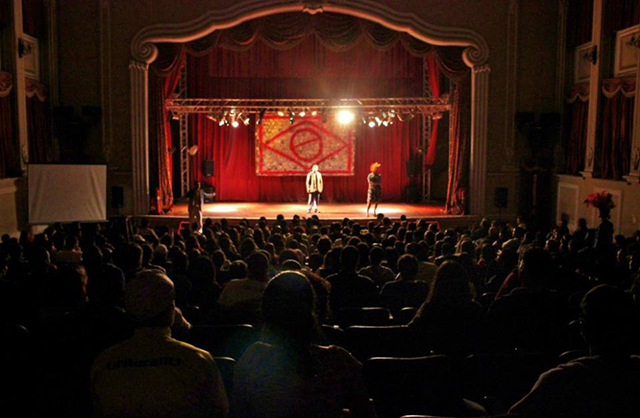
\includegraphics[width=250bp]{teatro.png}
\end{figure}
\begin{enumerate}

\item{}
Escreva duas equações que modelem as informações do enunciado. Quantas variáveis você necessita dispor para isso?

\item{}
Encontre três possibilidades para o número de ingressos vendidos de entrada cheia, meia entrada e de gratuidade que poderiam ter ocorrido, com as condições informadas no enunciado.

\item{}
Suponha que na noite do espetáculo, o número de pessoas com mais de 65 anos foi quatro vezes o número de aniversariantes. Quantos aniversariantes estiveram na plateia nesse dia?

\end{enumerate}


\ifdefined\prof
\begin{solucao}

\begin{enumerate}
\item Sejam $x,y$ e $z$ a quantidade de inteiras, meias e gratuidades, respectivamente, $x+y+z=500$ e $50x+25y=20500.$
\item Atividade exploratória, mas o professor pode pensar na solução da equação $50x+25y=20500$ considerando a restrição $x+y<500$.
\item $(350,120)$
\end{enumerate}

\end{solucao}
\fi

\end{document}